\documentclass[11pt]{article}

\usepackage[top=1in, bottom=1in, left=1in, right=1in]{geometry} 
\usepackage{graphicx}
\usepackage{titling}
\usepackage{float}
\usepackage{bm}
%\usepackage[fleqn]{amsmath}
\usepackage{amssymb,amsmath}
\usepackage{listings}
\usepackage{color}
\usepackage{enumitem}
\usepackage{fancyvrb}
\usepackage{hyperref}
\usepackage{setspace}
\usepackage{tabularx}
\usepackage{diagbox}
\usepackage{pdfpages}
\geometry{letterpaper}
\linespread{1.1}% \geometry{landscape} % rotated page geometry

\definecolor{codegreen}{rgb}{0,0.6,0}
\definecolor{codegray}{rgb}{0.5,0.5,0.5}
\definecolor{codepurple}{rgb}{0.58,0,0.82}
\definecolor{backcolour}{rgb}{0.95,0.95,0.92}
\definecolor{outcolor}{rgb}{0.545, 0.0, 0.0}

\lstdefinestyle{mystyle}{
	backgroundcolor=\color{backcolour},   
	commentstyle=\color{codegreen},
	keywordstyle=\color{magenta},
	numberstyle=\tiny\color{codegray},
	stringstyle=\color{codepurple},
	basicstyle=\footnotesize,
	breakatwhitespace=false,         
	breaklines=true,                 
	captionpos=b,                    
	keepspaces=true,                 
	numbers=left,                    
	numbersep=5pt,                  
	showspaces=false,                
	showstringspaces=false,
	showtabs=false,                  
	tabsize=2
}

\lstset{style=mystyle}

\setlength{\droptitle}{-5em}
\title{CE 264 Problem Set 5: Midterm Review}
\date{22 Mar. 2018} 
\author{Kun Qian \ \ \ \ \ \ (3033030782)\\ Franklin Zhao \ (3033030808)\\ Yichen Zhong \  (3033030873)}

\begin{document}
	
	\maketitle
	\renewcommand\theequation{\arabic{equation}}
	\renewcommand{\figurename}{Fig.}
	\renewcommand\thesection{Problem \arabic{section}}
	\renewcommand\thesubsection{(\Alph{subsection})}
	\renewcommand\thesubsubsection{Question (\alph{subsubsection}):}
	\onehalfspacing	
	
\section{}
\noindent The probability to move to North Berkeley is:
\begin{equation}\label{finaleq}
Pr(NB)=\frac{e^{V_{NB}}}{e^{V_{NB}}+e^{V_{SF}}+e^{V_{PO}}}\ \ \text{(since only 3 choices available here)}
\end{equation}
\noindent For the choice-residential model, we have the utility function:
\begin{equation}
U=\beta_{Rent}\times Rent+\beta_{Price}\times Price+\beta_{Size}\times Size+\beta_d\times DummyHouse+\beta_{Log}\times Logsum
\end{equation}
where most values are listed in the problem, but we still need to compute the logsum from the commuter's choice model.
\begin{equation}
LL=log(\prod Pr_{i,j})
\end{equation}
where $i\in\{1,2\}$ represents an individual; $j\in\{1,2,3\}$ represents a residence choice.\\\\
For a nested logit model:
\begin{align}
Pr(Driver)=Pr(Driver|Auto)\times Pr(Auto)\times...\\
Pr(Auto)=\frac{e^{\mu V_A}}{e^{\mu V_A}+e^{\mu V_N}+e^{\mu V_T}}\\ Pr(Driver|Auto)=\frac{e^{\mu_AV_D}}{e^{\mu_AV_D}+e^{\mu_AV_P}}\\
V_A=\frac{1}{\mu_A}log(e^{\mu_AV_D}+e^{\mu_AV_P})\ \ (\text{Similar for }\mu_{NM}\text{ and } \mu_T)
\end{align}
where $\mu_A=1.67$, $\mu_{NM}=1.205$, and $\mu_T=1.784$.
For each individual in each residential choice, the following utility equations are as follows:
\begin{equation}
V_{Drive}=ASC_{Drive}+\beta_{in-veichle}\times T_{Time}+\beta\times Cost
\end{equation}
\begin{equation}
V_{Passgr}=ASC_{ShareRide}+\beta_{in-veichle}\times T_{Time}+\beta\times Cost
\end{equation}	
\begin{equation}
V_{Walk}=ASC_{Walk}+\beta_{Walking}\times T_{Time}+\beta\times Cost
\end{equation}		
\begin{equation}
V_{Bike}=ASC_{Bike}+\beta_{Bike}\times T_{Time}+\beta\times Cost
\end{equation}	
\begin{equation}
V_{W-T}=ASC_{W-T}+\beta_{in-veichle}\times T_{Time}+\beta_{Wait}\times T_{Wait}+\beta_{Transit}\times T_{Transit}+\beta\times Cost
\end{equation}		
\begin{equation}
V_{A-T}=ASC_{D-T}+\beta_{in-veichle}\times T_{Time}+\beta_{Wait}\times T_{Wait}+\beta_{Transit}\times T_{Transit}+\beta\times Cost
\end{equation}	
The upper level utilites are computed in Table 1.
\begin{center}
Table 1: Upper level utilities
\end{center}
\begin{figure}[H]
\centering
\vspace{-0.6cm}    
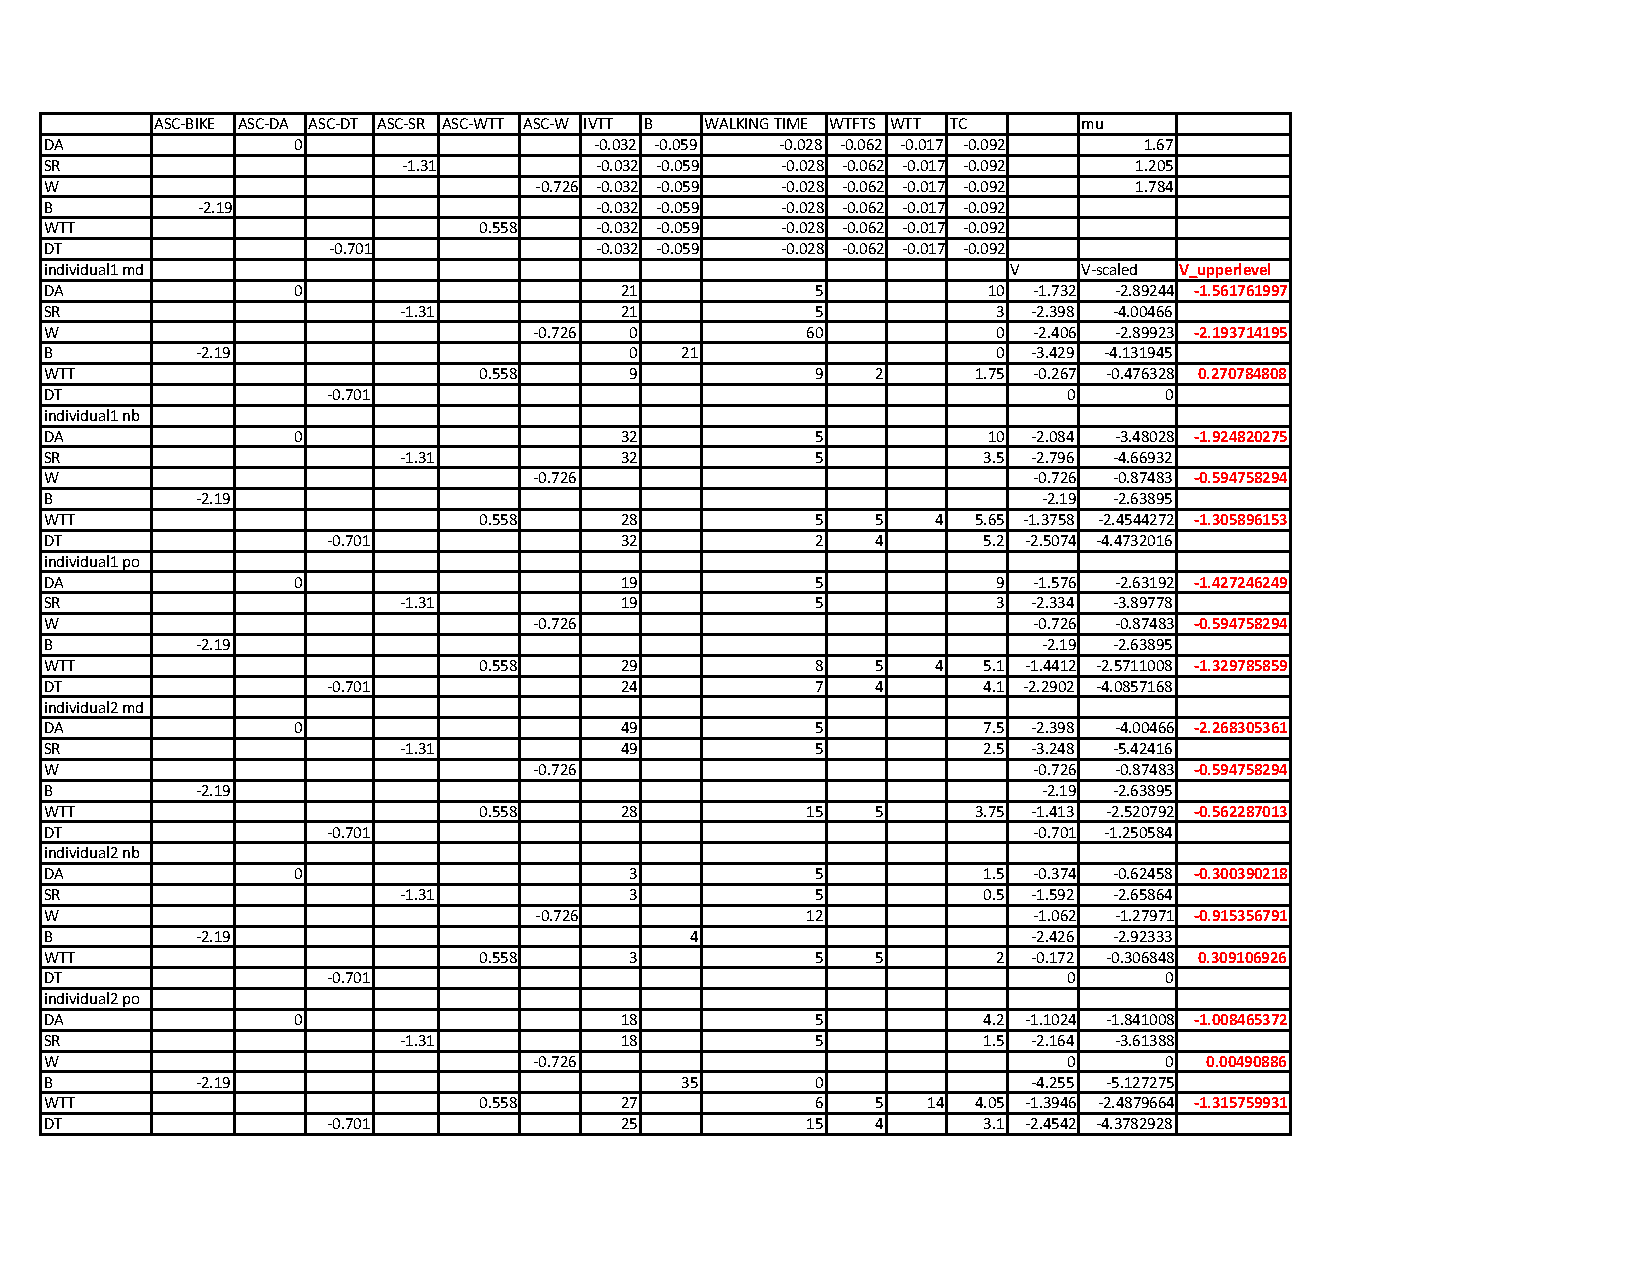
\includegraphics[width=\linewidth]{tb1.pdf}  
\end{figure}
Using these 12 computed upper level utilities, the following results can be derived:
\begin{align}
\tilde{V}_{MD,Auto}=log(e^{-1.562}+e^{-2.268})=-1.161\\
\tilde{V}_{MD,Non}=log(e^{-2.914}+e^{-0.595})=-0.411\\
\tilde{V}_{MD,Tran}=log(e^{0.271}+e^{-0.562})=0.632\\
\tilde{V}_{NB,Auto}=log(e^{-1.925}+e^{-0.300})=-0.121\\
\tilde{V}_{NB,Non}=log(e^{-0.595}+e^{-0.915})=-0.049\\
\tilde{V}_{NB,Tran}=log(e^{-1.306}+e^{0.309})=0.491
\end{align}
\newpage
\begin{align}
\tilde{V}_{PO,Auto}=log(e^{-1.427}+e^{-1.008})=-0.503\\
\tilde{V}_{PO,Non}=log(e^{-0.595}+e^{0.005})=0.443\\
\tilde{V}_{PO,Tran}=log(e^{-1.330}+e^{-1.316})=-0.630
\end{align}
Now, let's compute the logsum for each residential choice:
\begin{align}
\tilde{V}_{MD}=log(e^{-1.161}+e^{-0.411}+e^{0.632})=2.858\\
\tilde{V}_{NB}=log(e^{-0.121}+e^{-0.049}+e^{0.491})=3.472\\
\tilde{V}_{PO}=log(e^{-0.503}+e^{0.443}+e^{-0.630})=2.695
\end{align}
Hence, the utility for each residential choice can be derived:
\begin{align}
V_{MD}=-0.16\times29-0.064\times70+4.400\times0.82-0.782\times0+2.000\times2.858=0.204\\
V_{NB}=-0.16\times28-0.064\times60+4.400\times1.16-0.782\times1+2.00\times3.472=2.946\\
V_{PO}=-0.16\times18-0.064\times82+4.400\times1.26-0.782\times1+2.000\times2.695=2.024
\end{align}
Plug the above equations into Equation~(\ref{finaleq}), and the final result is obtained:
\begin{equation}
Pr(NB)=\frac{e^{2.946}}{e^{0.204}+e^{2.946}+e^{2.024}}=\bf{0.684}
\end{equation}
\section{}
\subsection{}
\begin{align}
Pr(P|G=1)=\frac{e^0}{e^{(0.3+1.8)}+e^1+e^0}=0.084\\
Pr(M|G=1)=\frac{(0.3+1.8)}{e^{(0.3+1.8)}+e^1+e^0}=0.687\\
Pr(T|G=0)=\frac{e^1}{e^{0.3}+e^1+e^0}=0.536\\
Pr(T|G=0)=\frac{e^0.3}{e^{0.3}+e^1+e^0}=0.266
\end{align}
\begin{equation}
LL=log(0.084^2\times0.687^4\times0.536^6\times0.266^2)=-12.8
\end{equation}
Hence, the value of the log-likelihood function at MLE is \textbf{-12.8}.
\subsection{}
\begin{equation}
\rho^2=1-\frac{L(\beta)}{L(0)}=1-\frac{-12.8}{14\times log(\frac{1}{3})}=1-\frac{-12.8}{-15.4}=\bf{0.17}
\end{equation}
\subsection{}
\textbf{Yes,} since now if we check the table of estimated parameters, we noticed given	that $\beta_{3T}=\beta_{3P}=0$, the graduate students' choice will always be $M$, which in fact makes $\beta_S$ not estimable. Hence, changing the availability like this would definitely affect the value of MLE.
\section{}
\subsection{}
\textbf{Yes.} Travel time is a variable across alternatives, so it can be included in all alternatives and four parameters can be estimable. In this example, the parameter values are partially constrained to be the same across motor and nonmotor alternatives.
\subsection{} 
\textbf{No.} Because the distance between home and destination for each staff is fixed and does not vary across alternatives. To modify the specification, estimated alternative-specific distance parameters and one base alternative can be used to replace a single beta for all four alternatives.
\subsection{} 
\textbf{No.} Because the average price per gallon is a fixed value for all respondents, which means it is perfectly correlated with the car constant. It can be modified to fuel cost per trip based on trip distances to estimate the parameter.
\subsection{} 
\textbf{Yes.} Female = 1 – Male. This variable does not vary across alternatives and it is categorical with two categories. So, one utility and one category must be the base and gender can be included in at most 3 alternatives. 
\subsection{} 
\textbf{No,} at most 2 variables can be included in each utility. So, one of the income categories need to be set as a base and drop from utility.
\section{}
\subsection{}
Because \textit{t-test}$=\frac{\hat{\beta}-0}{\bar{\sigma}}$,
\begin{equation}
\bar\sigma=\frac{\hat{\beta}-0}{\text{\textit{t-test}}}=\frac{0.8}{8.52}=0.094
\end{equation}
Then we let $\alpha$ walk-transit for Transit Nest to de a hypothesis test:
\begin{equation}
\begin{array}{rl}
H_0:&\alpha=1\\
H_1:&\alpha\neq1\\
\text{\textit{t-test}}=&\frac{0.8-1}{0.094}=-2.128<-2.1
\end{array}
\end{equation}
Thus we \textbf{reject} the null hypothesis, and the cross situation is preferred.
\subsection{}	
For unrestricted model, we can estimate much more parameters than restricted models. Thus, the likelihood and $\rho^2$ will increase, and we cannot confirm what happens to $\rho^2$.
\end{document}